\chapter{Analyse}

The following chapter presents a background research on the technologies
that can be used for graph exploration without the use of sight and a
description of the contributions from previous work of the HaptiQ. It
will first start with a task analysis on graph exploration. This chapter
aims at giving a wider outlook on the alternatives and additional
understanding on what characteristics should be considered for graph
exploration.

\section{Task analysis}\label{task-analysis}

Finding visually impaired people for collaboration with is not an easy
task. The partnership between IJA and ELIPSE tries to overcome this
issue, yet many different projects are running at the same time and each
one of them needs this worthy collaboration. In order to avoid constant
requests of their presence in the laboratories, ELIPSE has the
undergoing policy to restrict these requests to the evaluation phase.

This is a major drawback for a user centered development process.
Nevertheless, I have managed to find alternative sources of information
in order to acknowledge usability issues for visually impaired people.

\begin{itemize}
\item
  A direct contact with Bernard Orniola - one of the permanent members
  of ELIPSE who happens to be visually impaired. He has provided me with
  key understanding of this handicap in a day-to-day perspective
\item
  My tutor Christophe Jouffrais, who has a long experience in working
  with visually impaired people and was able to emphasize some aspects
  he could feel I was missing
\item
  My participation in general meetings on larger-scale projects such as
  AccessiMap has given me insight on how to adapt a development process
  to the needs of the blind
\item
  A direct contact with Ennadif Mustapha, who was doing his master internship in the
  cognitive science field. He has pointed out the limits of my design
  when I have exposed it to him
\item
  Colleagues who have tried a previous uncomplete version of the HaptiQ.
  They have warned me about the major issues that they have experienced
  when testing it.
\end{itemize}

This variety of intermediaries acted as a proxy for infield
observatories. Thanks to it, I was able to come up with the following
task analysis.

Giving a blind exploration using only a haptic device and a trained user
on the interaction techniques, the task would be decomposed into the
following steps:

\begin{enumerate}
\def\labelenumi{\arabic{enumi}.}
\item
  Feeling the device
\item
  Moving (depending on a possible strategy) and waiting for a feedback
\item
  If there is no tactile feedback, continue moving
\item
  If there is a tactile feedback, process to understand what the encoded
  information is
\item
  Given the new piece of information acquired, adapt the strategy of
  exploration
\item
  While exploration is not completed go back to step 2
\end{enumerate}

These steps may seem fairly simple, yet they give us some clues on the
importance of having a recognisable tactile signal during the
explroation phase.

Another interesting aspect is the fact that an exploration is the result
of a sum of strategies. We can consider that finding the network is the
first goal. The next one is to explore all the nodes, which can mean
following the network as much as possible. A possible solution to
improve this strategy may involve building tactile signals that would
naturally suggest strategies and assist the users in their choices.

\section{Related research}\label{related-research}

Making an exhaustive taxonomy would be illusionnary as research related
to haptics devices has extended its scope and depth over the last twenty
five years \cite{roberts2007we}. This chapter will nevertheless attempt to
present technologies that could be used as a way to acquire data through graphs or
maps for the sightless.

This background research is based on the doctoral thesis of
Thomas Pietrzak on ``Dissemination of haptics information in a
multimodal environnement'' \cite{pietrzak:tel-00390057} and on the master thesis of Conte Simone on
``The HaptiQ: A Haptic Device for Graph Exploration by People with Visual Disabilities''.

\subsection{Braille}\label{braille}

Braille is a tactile writing system that has been invented in 1824 and
then spreaded around the world since. Although it could be used to read
graphs with series of dots, arrows and bullets, it is intended for text
reading. The main issue remains the fact that it is difficult to learn.
Thinking that all blind people would know it is a common misconception.

\subsection{ScreenReaders}\label{screenreaders}

VIP rely heavily on their audition in order to compensate for their
handicap. This usage would even trigger an ``obstacle perception'' in
which they would feel object just by hearing sounds \cite{levesqueblindness}.
ScreenReaders provides an efficient alternative to access text and many
are available \footnote{\url{http://alternativeto.net/tag/screen-reader/}
  (accessed the 19/08/15)}. If only a few screen readers would allow
navigation tasks as well, like JAWS\cite{JAWS} or VoiceOver\cite{voiceOver}, the main issue remains
the usage of audio as a channel for spatial guidance. VIP are not
necessarily inclined to use either cardinal points or the four
directions (up, down, right, left) to orient themselves. That is why map
exploration through a screen reader would require a constant audio
feedback. This interaction may provide a useful help for graph
exploration, yet it cannot be qualified as the most suited. Besides, it
is preferable to interfer with the audio channel as little as possible
in order to facilitate the debit of textual information expressed this
way. In other words, it would be beneficial to fill this channel with
textual and mainly textual information.

	\begin{figure}[!ht]
		\begin{minipage}[c]{.46\linewidth}
			\centering
			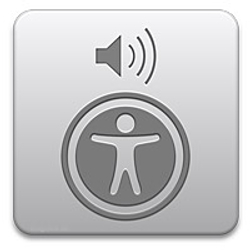
\includegraphics[width=4cm]{figures/voice_over.jpg}
			\caption{Voiceover icon, the screen reader made by Apple}
  		\end{minipage} \hfill
  		\begin{minipage}[c]{.46\linewidth}
  			\centering
			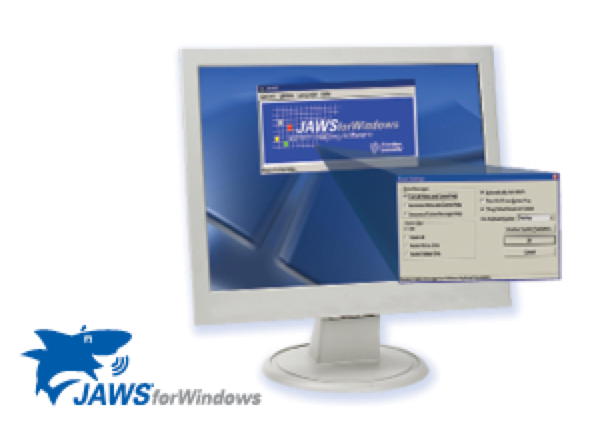
\includegraphics[width=6cm]{figures/jaws.png}
			\caption{Jaws, the screen reader made by Windows}
		\end{minipage}
	\end{figure}

\subsection{Tactile Maps}\label{tactile-maps}

Tactile maps are made of paper heated to form bumps and relief. It thus
creates shapes, lines and dots. These are popular among visually
impaired people learning geometry or exploring a map. Even though they
offer plenty of tactile freedom, it is easier to grasp a general idea of
the shapes by using the ten fingers. They do not provide further
interaction unless they are combined with a tabletop such as the
Multimodal Interactive Maps (MIMs) project \cite{brock2010usage}. MIMs is an input
output system mixing different technolgies. It keeps the possibility of
a ten fingers exploration, but requires a new printing for each
visualisation. MIMs fall short of rendering VIPs autonomous: scanning
and printing would require the help of another person.

	\begin{figure}[!ht]
		\centering
		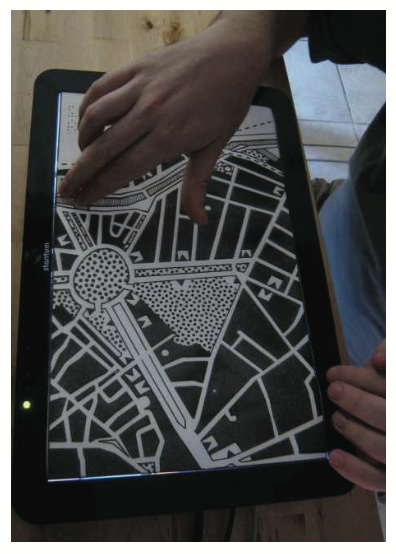
\includegraphics[height=5cm]{figures/mims.png}
		\caption{A MIM prototype in use}
	\end{figure}


\subsection{Machanical actuators}\label{machanical-actuators}

Presented as the technologic equivalency of braille,
they can dynamically change a matrix of actuators in order to provide information
which can be a Braille symbol or simple shapes. This matrix can be
placed on the finger zone of a mouse like the VTPlayer
or the Tactiball \cite{Lecolinet:2005:TOC:1148550.1148583} which implies that the moving hand is
also receiving the tactile information or it can be separated like the
Tactos device \cite{hanneton1998dynamique} but with a smaller matrix. Their lack of
popularity could result from poor quality software applications, as
Thomas Pietrzak suggests. Given Jansson study \cite{jansson2005obtaining} mouses are not
compatible with navigation tasks for visually impaired people.

\begin{figure}[!ht]
	\begin{minipage}[c]{.32\linewidth}
		\centering
		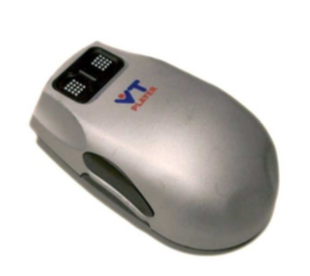
\includegraphics[width=3cm]{figures/vtplayer.png}
		\caption{VTPlalyer}
		\end{minipage} \hfill
	\begin{minipage}[c]{.32\linewidth}
			\centering
		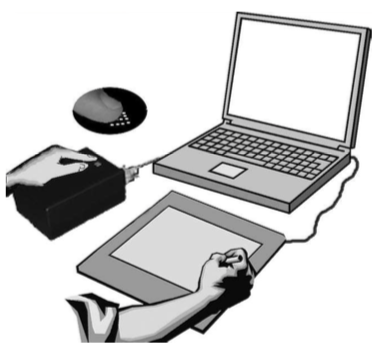
\includegraphics[width=3cm]{figures/tactos.png}
		\caption{Tactos}
	\end{minipage}
	\begin{minipage}[c]{.32\linewidth}
		\centering
		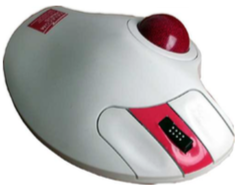
\includegraphics[width=3cm]{figures/tactiball.png}
		\caption{Tactiball}
	\end{minipage}
\end{figure}

Other displays, like the Brailliant from Humanware \cite{HumanWare},
offer a full range of actuators forming braille letters, but remain
fairly expensive.

HTP, a precursor of the HaptiQ, deserves particular attention. One of my
tutors -- Miguel Nacenta, has been involved in the design of this
input/output device with a single actuator in the center \cite{marquardt2009haptic}. The purpose of the HTP is to explore other possible
interactions with tabletops like their further work has suggested \cite{ledo2012haptictouch}. It renders unconventional outputs like friction and softness ~\ref{fig:puck-d}
which can be integrated in various applications. Although innovative,
its usage is supported by visual elements ~\ref{fig:puck-visual} and has not been though threw
for visually impaired people.

\begin{figure}[!ht]
	\begin{minipage}[c]{.45\linewidth}
		\centering
		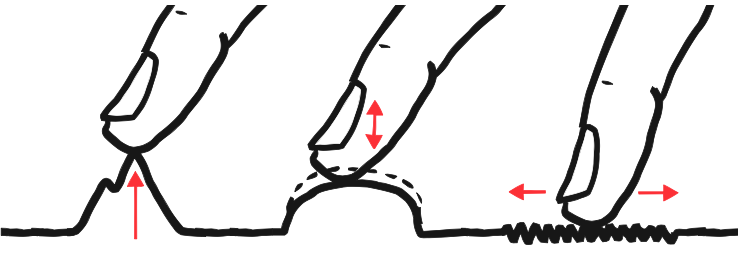
\includegraphics[width=5cm]{figures/puck-d.png}
		\caption{The Haptic Table Top Puck innovative outputs \label{fig:puck-d}}
	\end{minipage}
	\begin{minipage}[c]{.45\linewidth}
		\centering
		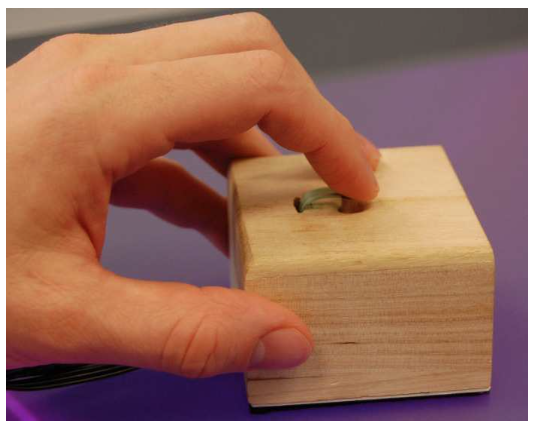
\includegraphics[width=3cm]{figures/puck-image.png}
		\caption{The Haptic Tabel Top Puck has one center actuator}
	\end{minipage}
\end{figure}

\begin{figure}[!ht]
	\centering
	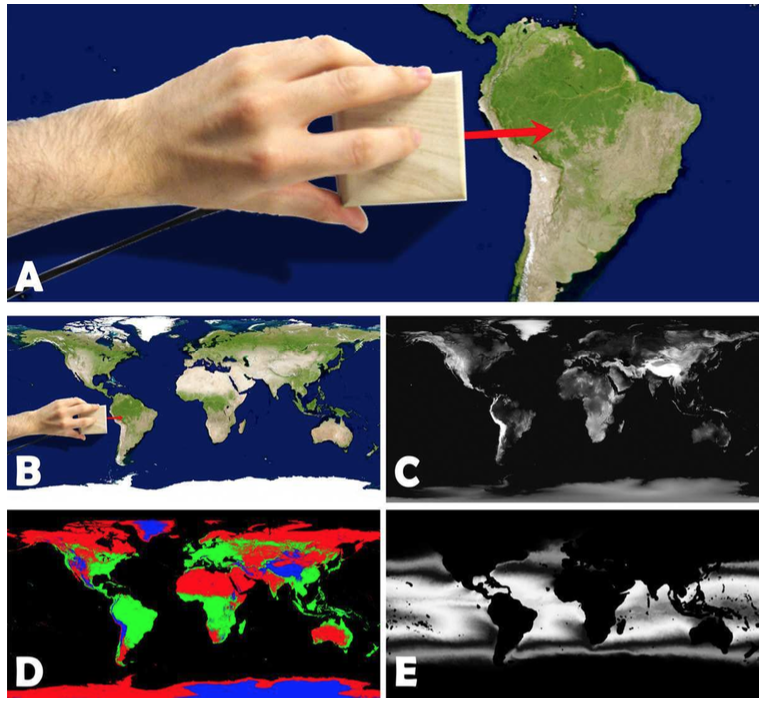
\includegraphics[height=5cm]{figures/puck-visual.png}
	\caption{The Haptic Table Top Puck interacts well with tabletops, but its usage requires visual support \label{fig:puck-visual}}
\end{figure}

% \caption{Bake options with CakePHP\label{fig:cakePHP-option}}
% figure ~\ref{fig:cakePHP-option}.

\subsection{Vibrations}\label{vibrations}

Some devices use vibrations in oder to provide feedbacks. Small
vibro-motors can be attached to a glove which makes the device adapted
to a hand like the Cybertouch glove \cite{astrauskas2008cybertouch}. They could also be
integrated on a small surface imitating a matrix of actuators like the
Optacon \cite{linvill1966direct}.

Vibrations can be used in a matrix of thin vertical panels trigerring a
feeling of cavity or bumps when a hand is set on it as in STReSS and its second version STReSS 2 \cite{wang2006compact}.

Electrovibration is used in the TeslaTouch and Revel systems \cite{bau2010teslatouch, bau2012revel}; it is imitating the sensation of friction and is therefore only perceptable when the fingers are in motion which would be incompatible with our task analysis done previously.

\begin{figure}[!ht]
	\begin{minipage}[c]{.45\linewidth}
		\centering
		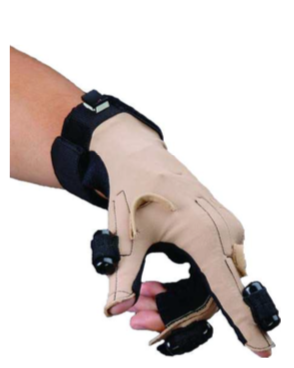
\includegraphics[height=5cm]{figures/cybertouch.png}
	\caption{The cybertouch glove}
	\end{minipage}
	\begin{minipage}[c]{.45\linewidth}
		\centering
		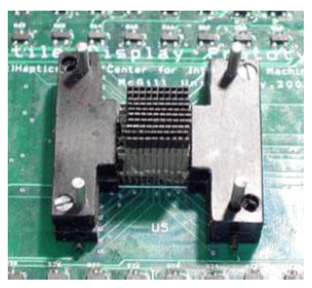
\includegraphics[width=5cm]{figures/stress.png}
		\caption{Stress uses vertical panels to vibrate in order to create a sensation of bumps}
	\end{minipage}
\end{figure}

\begin{figure}[!ht]
	\centering
	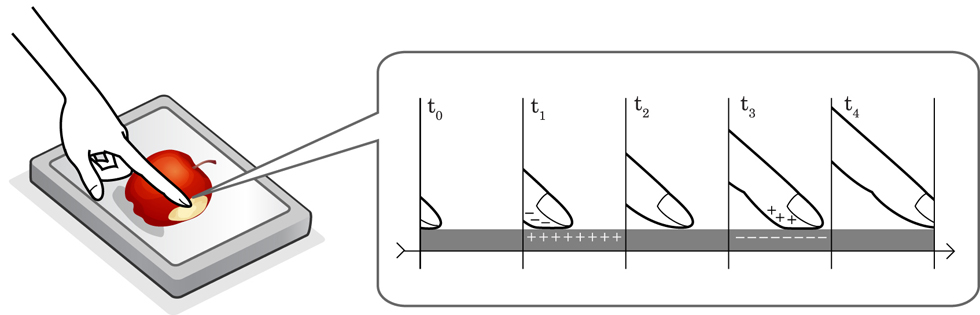
\includegraphics[width=8cm]{figures/teslatouch.png}
	\caption{The TeslaTouch}
\end{figure}


\subsection{Forcefeedback}\label{forcefeedback}

Forcefeedback has known a famous entry in the gaming field with Joystick
and Wheels. But their application goes far beyond that. One of the most
recurrent names is the PHANToM \cite{massie1994phantom} that forces the point in
certain directions. Forcefeedback comes in a variety of techniques in
order to push a single point into a certain direction (articulated arm,
pantographes, or pneumatics).

Having a single point of contact does not allow users to follow lines
easily orto understand shapes \cite{yu2001haptic}. This make Forcefeedback
unsuitable for our project.

\begin{figure}[!ht]
	\centering
	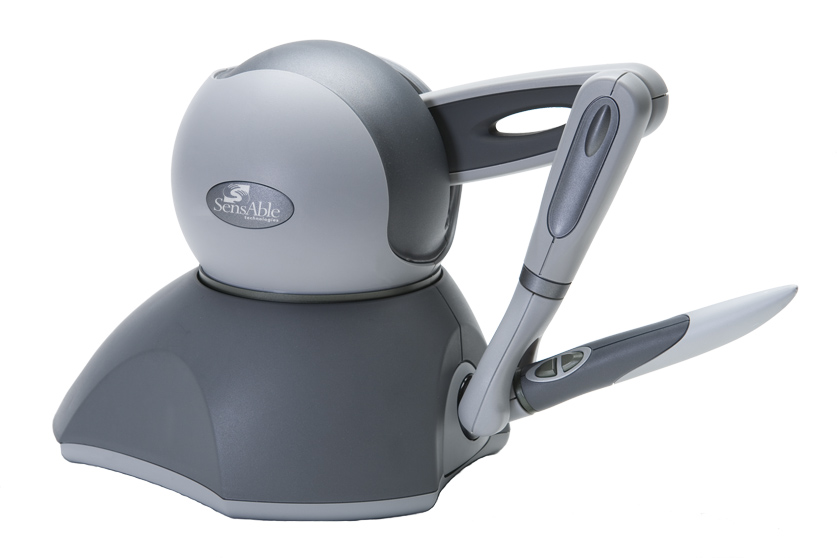
\includegraphics[height=4cm]{figures/phantom.png}
	\caption{PHANToM makes a strange sensation when the user tries to go through a virtual object}
\end{figure}

\subsection{Air}\label{air}

Feedbacks can be perceived via air motion. It triggers the same signals
as with tactile motion thanks to the variety of sensitivy receptors \cite{klatzky1999zl}. AIREAL \cite{sodhi2013aireal} makes this approach possible and uses a
motion detector camera as input. Using highly pressured air waves allows
long distance interaction (10m). Besides, it is scalable and affordable.
Even though they offer a wide range of angles from which the air is
pushed, the lack of resolution limits its usage tremendously. Plus,
AIREAL is presented as an interaction more suited to enhance user
experience than an input output system for exploration.

\begin{figure}[!ht]
	\centering
	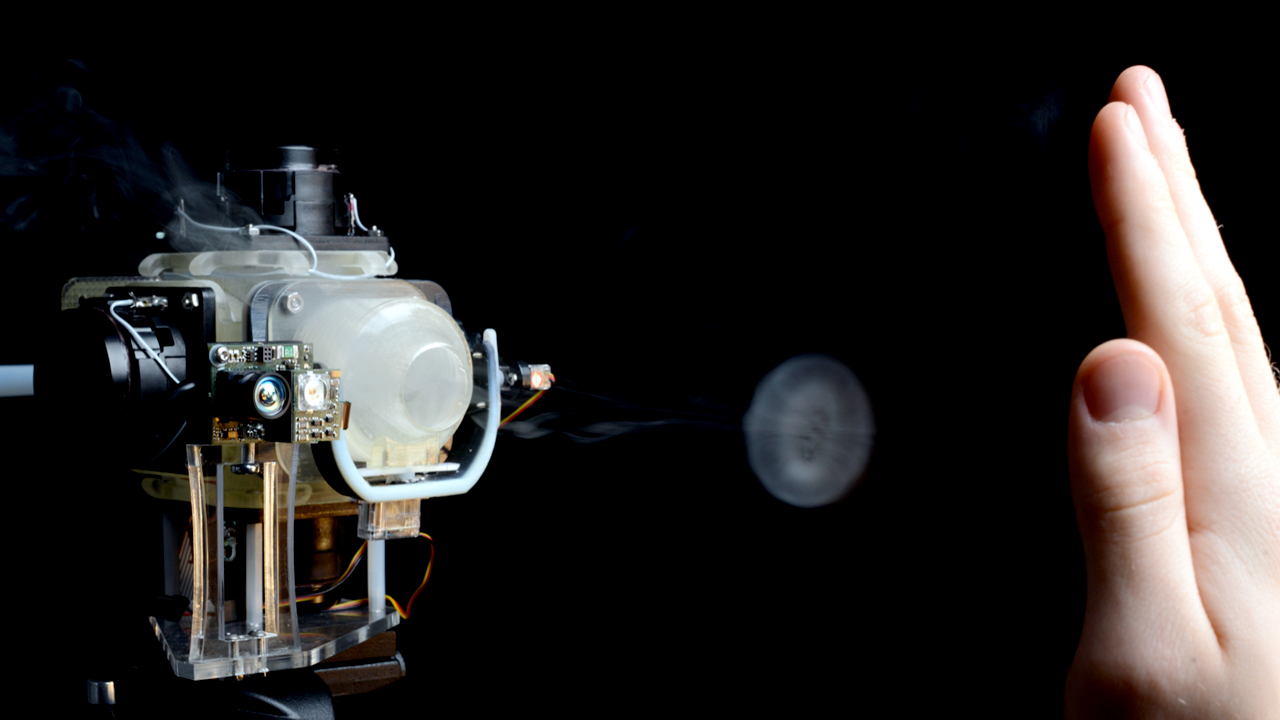
\includegraphics[height=5cm]{figures/aireal.png}
	\caption{AIREAL creates an air vortex perceptible}
\end{figure}

\subsection{No hands involved}\label{no-hands-involved}


\begin{figure}[!ht]
	\centering
	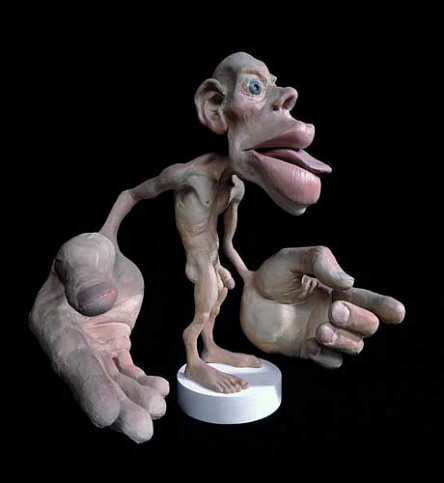
\includegraphics[height=5cm]{figures/sensory_homunculus.png}
	\caption{The Sensory Homunculus from the Natural History Museum of London \cite{homonculus}}
\end{figure}

If we were to represent the human body by its touch sensitivity, we would
end up with a weak figurine with enormous hands, lips and tongue. This
is maybe why bolder interactions are exploiting the latter with the
Tongue Display Unit \cite{bach1998form}. This display places a seven by seven grid
filled with electrodes on the tongue and can be used in a
no-hands-involved scenario: as for instance a working surgeon. Others
would use the brow with the Forhead Retina System \cite{kajimoto2006forehead}.

Although intriguing, both of these displays allow limited interaction
and are suited for very particular scenarios.

\begin{figure}[!ht]
	\centering
	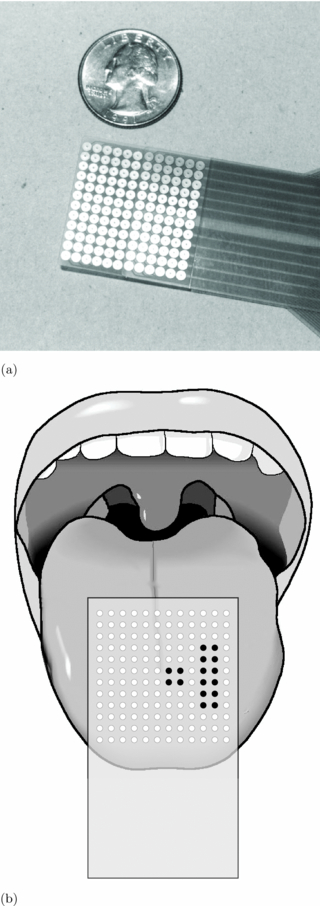
\includegraphics[height=5cm]{figures/tongue_display_unit.png}
	\caption{The Tongue Display Unit}
\end{figure}

\section{Previous versions}\label{previous-versions}

\begin{figure}[!ht]
	\begin{minipage}[c]{.45\linewidth}
		\centering
		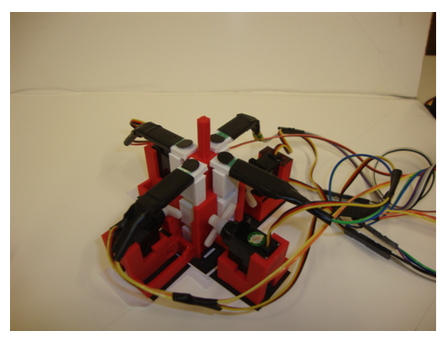
\includegraphics[width=5cm]{figures/simone_haptiq_4.png}
		\caption{The HaptiQ with four actuators}
	\end{minipage}
	\begin{minipage}[c]{.45\linewidth}
		\centering
		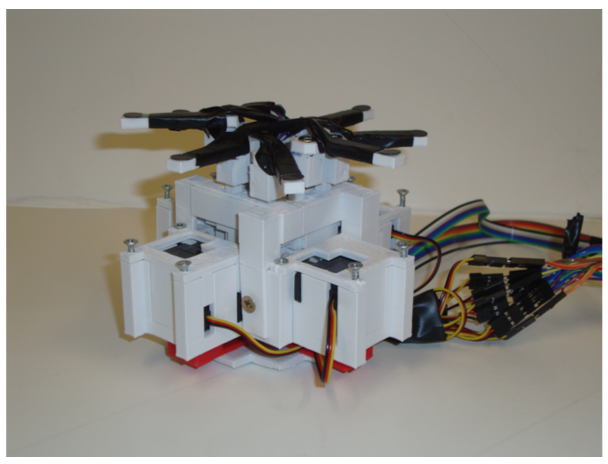
\includegraphics[height=5cm]{figures/simone_haptiq_8.png}
		\caption{The HaptiQ with eight actuators}
	\end{minipage}
\end{figure}

In 2014, Constan Simone has worked on a first version of HaptiQ at the
University of St Andrews. His development process was focused on the
engineering of a device to handle multiple actuators. These actuators
could therefore have their own language in order to transmit
information. He has designed multiple cases for the HaptiQ and
maintaining all the servomotors.

His work on a background research narrowed the disadvantages of other
haptics solutions. He has also implied that a vector based mechanical
actuator such as the HaptiQ is unique. His ideas on possible
applications in order to help math signal representation as in Figure ~\ref{fig:simone-math} are highly valuable.

\begin{figure}[!ht]
	\centering
	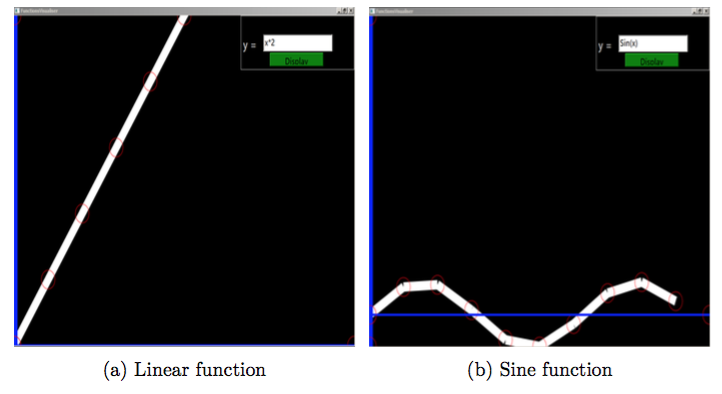
\includegraphics[height=5cm]{figures/simone_maths.png}
	\caption{A maths application that turns simple equations into graph\label{fig:simone-math}}
\end{figure}

Even though his design on the caps does not appear in his report, we
have to give him credit for it. His work on tactons seems promising;
yet, it is not backed up by any user study. This imposes its
reconsideration.

Simone has also managed to extend this first version with button and has
started to work on different possible interactions with pressure.

Finally, he has briefly pointed out the issue of having multiple wires
running in order to control the servomotors which has led me to prefer
solutions allowing the device to be as nomad as possible.

\section{Conclusion}\label{conclusion}

Haptics devices demand material and often electronic circuits to be
build. This results in high costs overall and is often dedicated to a
specific usage. If our goal is to provide a solution for VIP around the
world, then we should take into account other aspects such as making it
easily replicable and allowing applications to be build on top of the
key interactions like the Haptic Puck Tabletop and the Phantom did and just like Simone started. But
this goal requires various skills and careful designs.

Many alternatives exist, but the same issue remains: we are too focused
on data representation than on data meaning. It might be more relevant to
focus on the general trends than on the exact measurements \cite{roberts2007we}. Let us
remember that it is really hard to learn the simple concept of a squared
angle when one would be deprived of sight. The challenge is there:
trying to give a natural interaction for the strategies involved in
exploration and facilitate learning. A way of solving it is to take a
step back in the representation of information: we are not interested in
the value of a particular pixel but its meaning, its purpose. Is it a
part of an edge? Is it filling a cue point? Or is it just random noise?
These problems can be solved by giving meaning to a particular point; this
is why we are focusing only on graphs. They are a scalable and precise
representation of the key information. Understanding graphs is mastering
a way to easily acquire conceptual and spatial information.